\chapter{基礎知識}
本章では,量子回路,量子ゲートとビームサーチの基礎知識について説明する.
\section{量子回路}
量子回路は,量子計算\cite{deutsch1985quantum}を
量子ゲートと量子ビットを用いて表したものである.
量子ビットと量子ゲートは従来の計算機におけるビットと論理ゲートに相当する.
量子ゲートは従来の論理ゲートと同様に入力と出力を持つ.
複数の量子ゲートを組み合わせることで目的の演算を実現することができる.
量子回路は常に可逆性を持たなければならないという,論理回路とは異なる性質を持つ.
つまり,量子回路は出力から入力が一意に求めることができなければならない.
\par 
\begin{figure}[tbp]
  \centering
  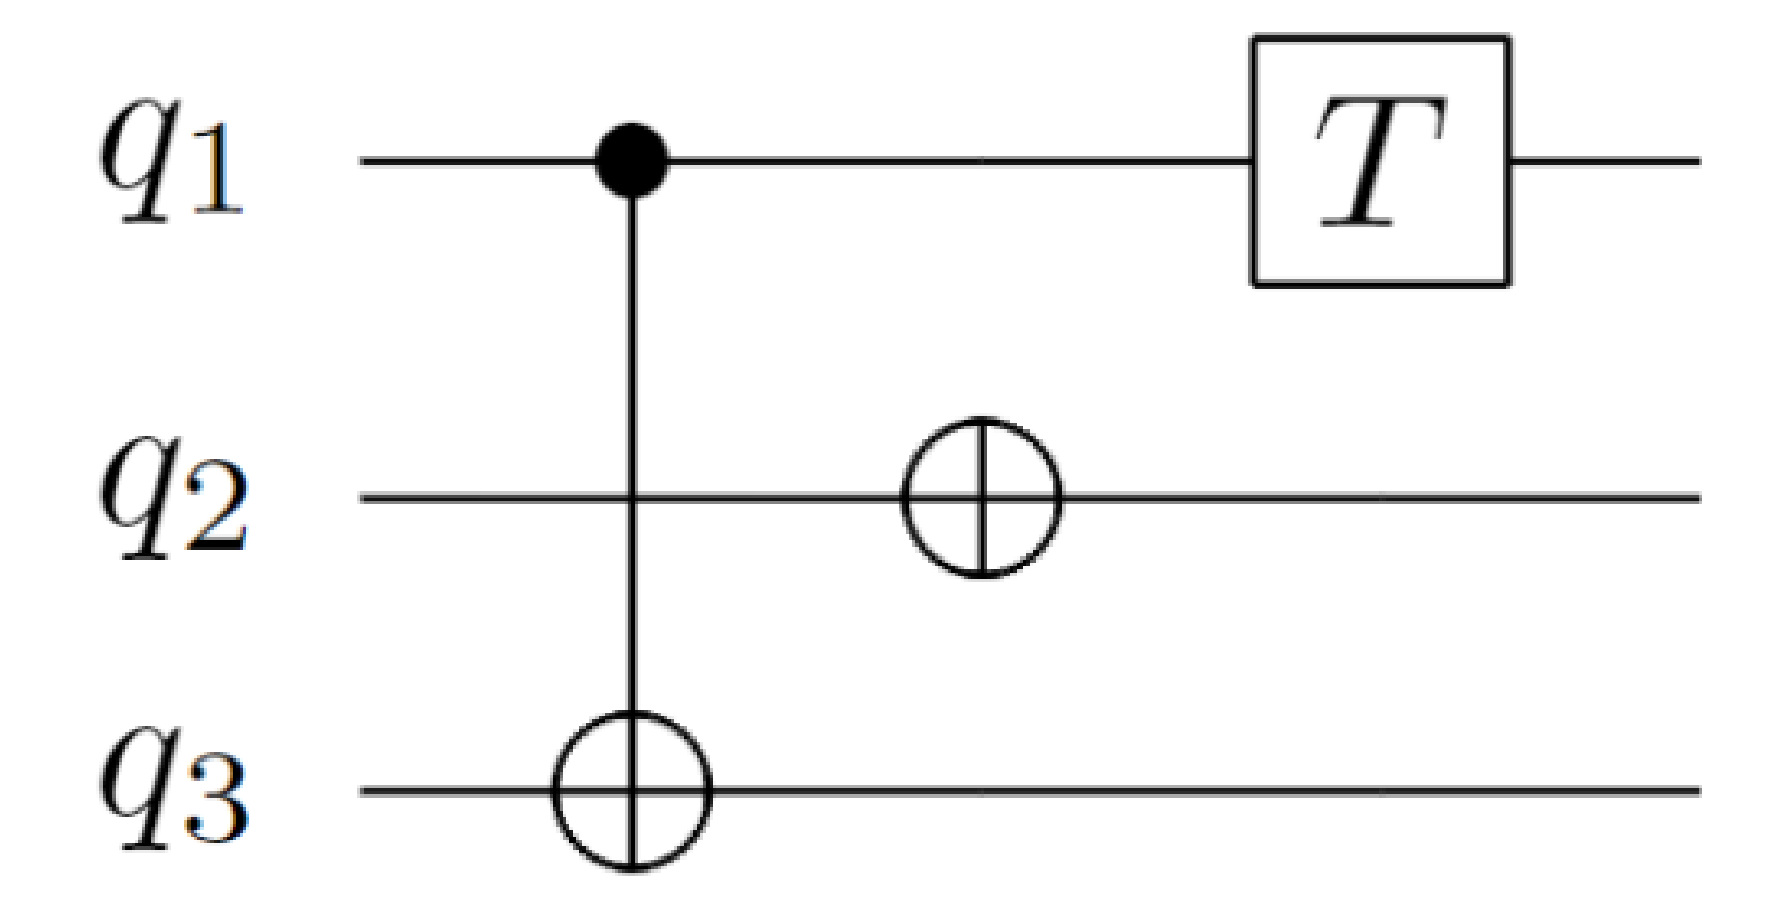
\includegraphics[width=7cm]{img/qcircuit.pdf}
  \caption{量子回路の例}
  \label{qcircuit}
\end{figure}
量子回路の例を図~\ref{qcircuit}に示す.
図~\ref{qcircuit}中の$q_{1}$,$q_{2}$,$q_{3}$というラベル付けされた横線は
量子ビットを表す.
量子ゲートは,図~\ref{qcircuit}のように各ゲートに対応するシンボルで図示される.
量子回路は左側が入力で右側が出力である.
そのため,量子ゲートは左のゲートから順に実行される.
\section{量子ゲート}
量子ゲートは,量子ビットの量子状態を変化させる機能をもつ.
量子ゲートは量子ビットを入力に持ち,コントロールビットとターゲットビット
で構成される.量子ゲートの中にはコントロールビットを持たないものも存在する.
コントロールビットは,量子ゲートをターゲットビットに作用させるかどうかを判定する
量子ビットである.
コントロールビットの値が1のとき,量子ゲートをターゲットビットに作用させる.
一方,ターゲットビットは,コントロールビットの条件が満たされると,
量子ゲートの演算結果によって状態が変化させられる量子ビットのことである.
\par
量子ゲートにはClifford+T\cite{zhou2000methodology}と呼ばれる
$NOT, CNOT, H, T,T^{\dagger}$ゲートからなるゲート群がある.
\gout{エラー訂正を行いながら所望の計算を行う,フォールトレラントな量子計算の枠組みで,}
演算を行うにはこのClifford+Tのゲート群に量子ゲートを分解する必要がある\cite{boykin2000new}.
\par
\bout{量子ゲートが量子ビットに対して行った操作を元に戻す操作のことを逆変換と呼ぶ.
逆変換を行う量子ゲートは,$\dag$を付けて表すことができる.
例えば,$T$ゲートの逆変換は$T^{\dag}$ゲートである.
$T$ゲートを作用させた後に$T^{\dag}$ゲートを作用させると,
$T$ゲートを作用させる前の状態に戻すことができる.}
\subsection{NOT ゲート}
NOT ゲートは従来の計算機の NOTゲートと同じ機能を持つ.NOT ゲートの例を
図~\ref{not_gate}に示す.NOTゲートは1量子ビットのターゲットビットのみで構成されたゲートである.
NOTゲートはターゲットビットの値が$0$ならば$1$を出力し,$1$ならば$0$を出力する.
\begin{figure}[tbp]
  \centering
  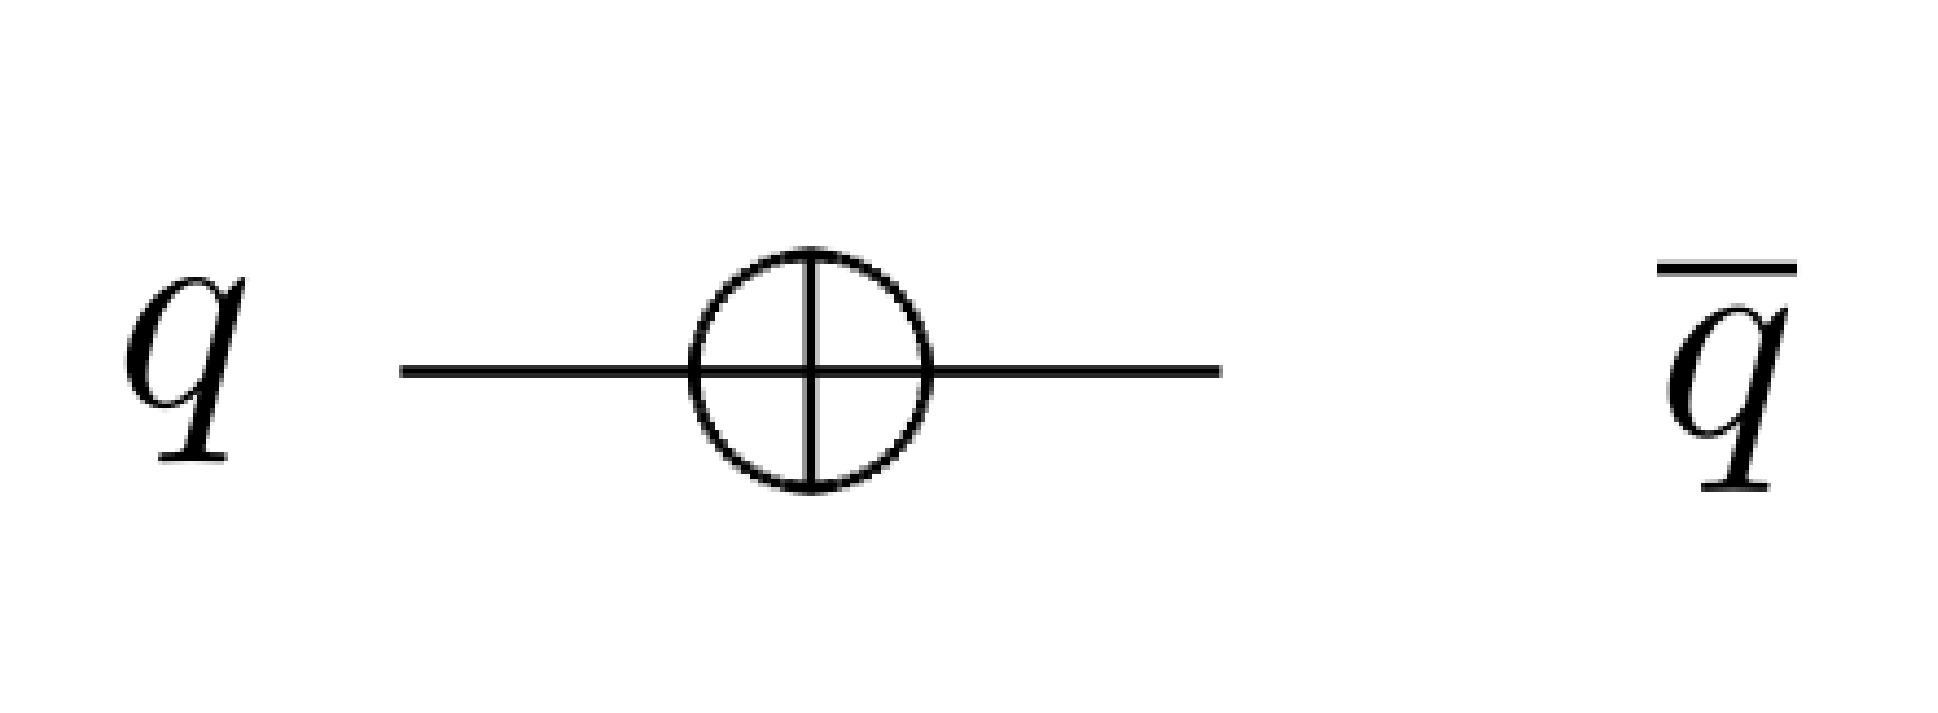
\includegraphics[width=7cm]{img/notgate.pdf}
  \caption{NOTゲート}
  \label{not_gate}
\end{figure}
\subsection{CNOTゲート}
CNOTゲートは1つのコントロールビットと1つのターゲットビットで
構成された量子ゲートである.
CNOTゲートの例を図~\ref{cnot_gate}に示す.
\begin{figure}[tbp]
  \centering
  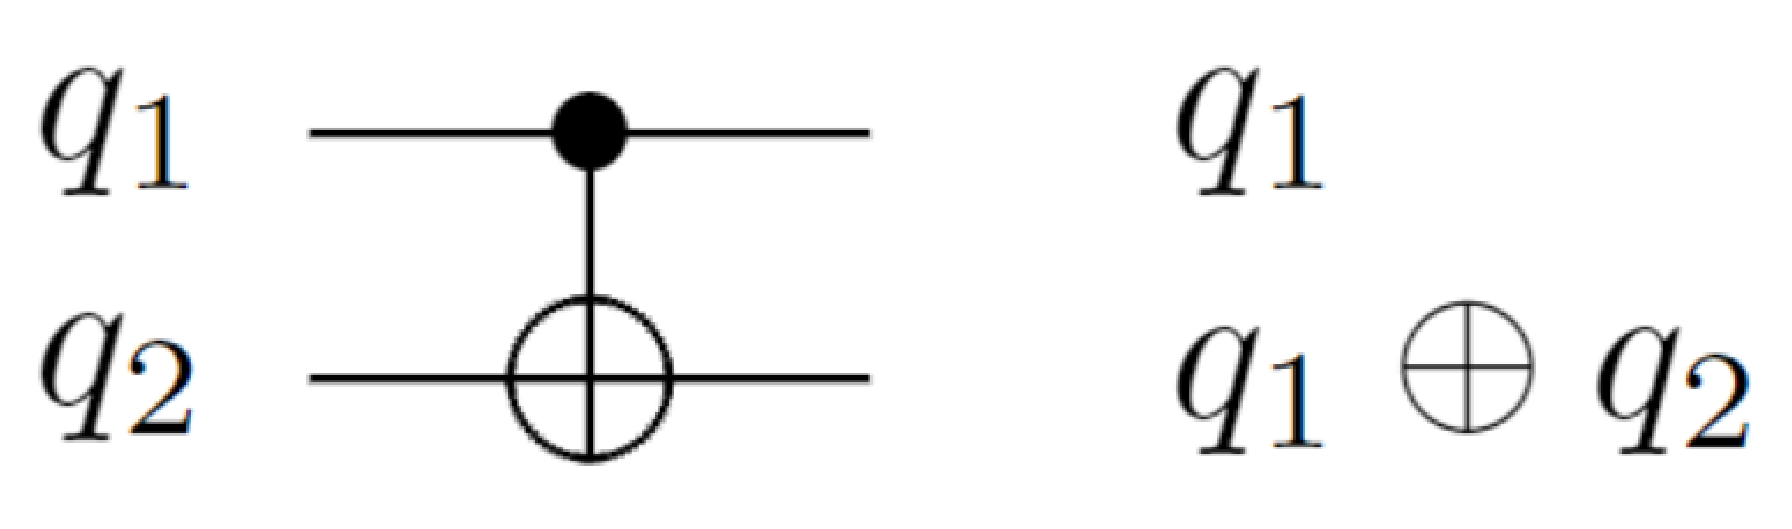
\includegraphics[width=8cm]{img/cnotgate.pdf}
  \caption{CNOT ゲート}
  \label{cnot_gate}
\end{figure}
図~\ref{cnot_gate}中の黒丸●をコントロールビットと呼び,
$\oplus$をターゲットビットと呼ぶ.
CNOTゲートはコントロールビットの値が0のときターゲットビットを変化させず,1のときターゲットビットを反転させる.
コントロールビットの値は変化することはないため,
量子ビット$q_{1}$の値はCNOTゲートを通過しても変化しない.
\subsection{Tゲート}
\bout{$T$ゲートは,作用させる量子ビットの値が1のとき,}
量子状態の位相を$\frac{\pi}{4}$変化させる1量子ビットの量子ゲートである.
\bout{また,$T$ゲートの逆変換を$T^{\dag}$ゲートと呼ぶ.}
\bout{$T^{\dag}$ゲートは$T$ゲートの逆変換であるため,作用させる量子ビットの値が1のとき,
量子状態の位相を$-\frac{\pi}{4}$変化させる.}
$T$ゲート,$T^{\dag}$ゲートの例を図\ref{T_T_dag}に示す.
\begin{figure}[tbp]
  \centering
  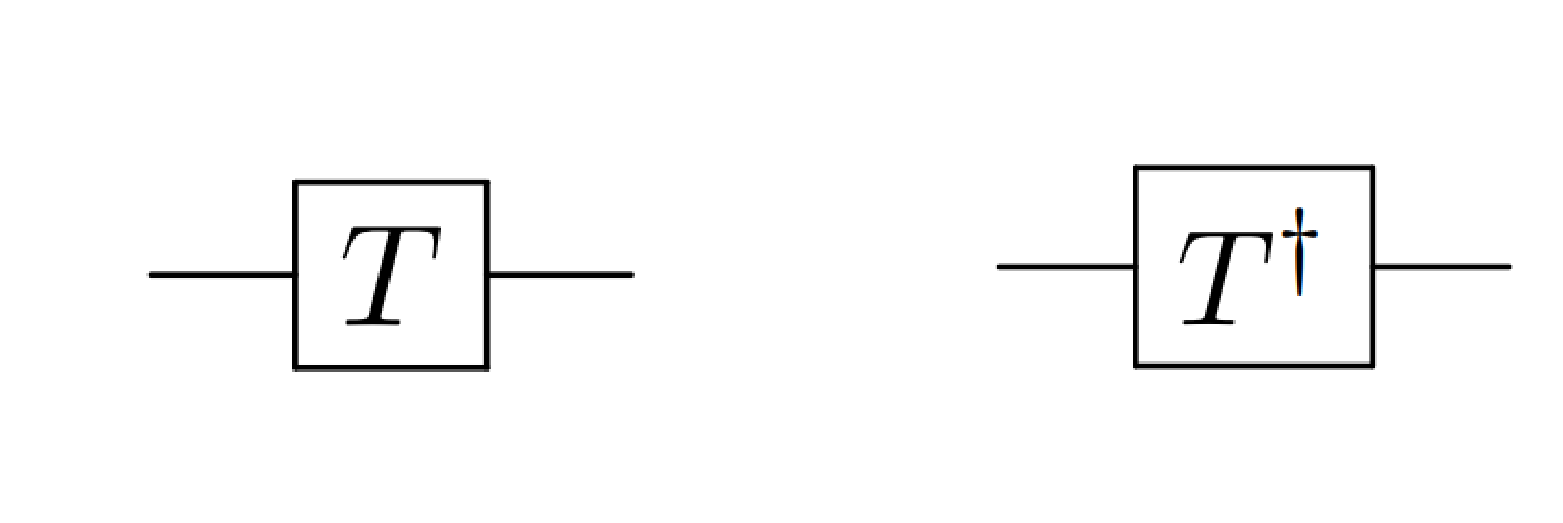
\includegraphics[width=7cm]{img/T_T_dag.pdf}
  \caption{$T$ゲート,$T^{\dag}$ゲート}
  \label{T_T_dag}
\end{figure}
\par
$T$ ゲート,$T^{\dagger}$ゲートの操作時間は他のClifford+Tのゲート群の量子ゲートと比較して非常に長い\cite{fowler2009high}.
そのため,量子回路中の同時に実行できない$T$ゲート,$T^{\dag}$ゲートの段数をT-depth\cite{amy2013meet}と呼び,
T-depthの値を削減することが,量子回路設計の課題とされている.
本論文ではT-depthのみを考慮するため,$T$ゲート,$T^{\dag}$ゲートをまとめて$T$ゲートと呼ぶ.
\subsection{Toffoliゲート}
Toffoliゲートは3量子ビットの量子ゲートである.
Toffoliゲートは,2つのコントロールビットと1つのターゲットビットで構成される.
Toffoliゲートは,すべてのコントロールビットの値が1であるとき,ターゲットビットの値を反転する.
Toffoliゲートの演算を実現するには,Clifford+Tのゲート群に分解する必要がある.
図~\ref{toffoli}にToffoliゲートとその分解例を示す\cite{amy2013meet}.
\par
図~\ref{toffoli}の分解例では,同時に実行できない$T$ゲートが3段現れる.
このため,図~\ref{toffoli}のToffoliゲートのT-depthは3となる.
\begin{figure}[tbp]
  \centering
  \includegraphics[width=11cm]{img/toffoli.pdf}
  \caption{ToffoliゲートとClifford+Tへの分解例\cite{amy2013meet}}
  \label{toffoli}
\end{figure}
\subsection{Multiple Controlled Toffoli(MCT)ゲート}
Toffoliゲートを一般化したものをMultiple Controlled Toffoli(MCT)ゲート\cite{barenco1995elementary}と呼ぶ.
MCTゲートは複数のコントロールビットと1つのターゲットビットで構成される.
MCTゲートはすべてのコントロールビットの値が1のとき,ターゲットビットビットの値を反転する.
\par
MCTゲートもToffoliゲートと同様にClifford+Tのゲート群に分解する必要がある.
コントロールビット数が3個以上の
MCTゲートを分解するには,
補助ビットと呼ばれる値を一時的に保存するビットを使用する必要がある.
ここで使用した補助ビットは,値を復元する必要がある.
\gout{MCTゲートは,}
補助ビットを用いずにClifford+Tに分解できるゲート,
例えばToffoliゲートに,\gout{一度分解される.}
そして,分解したゲートをClifford+Tのゲート群に分解する.
\par
図~\ref{barenco}にコントロールビット数が4個のMCTゲートのToffoliゲートへの分解例を示す.
\begin{figure}[tbp]
  \centering
  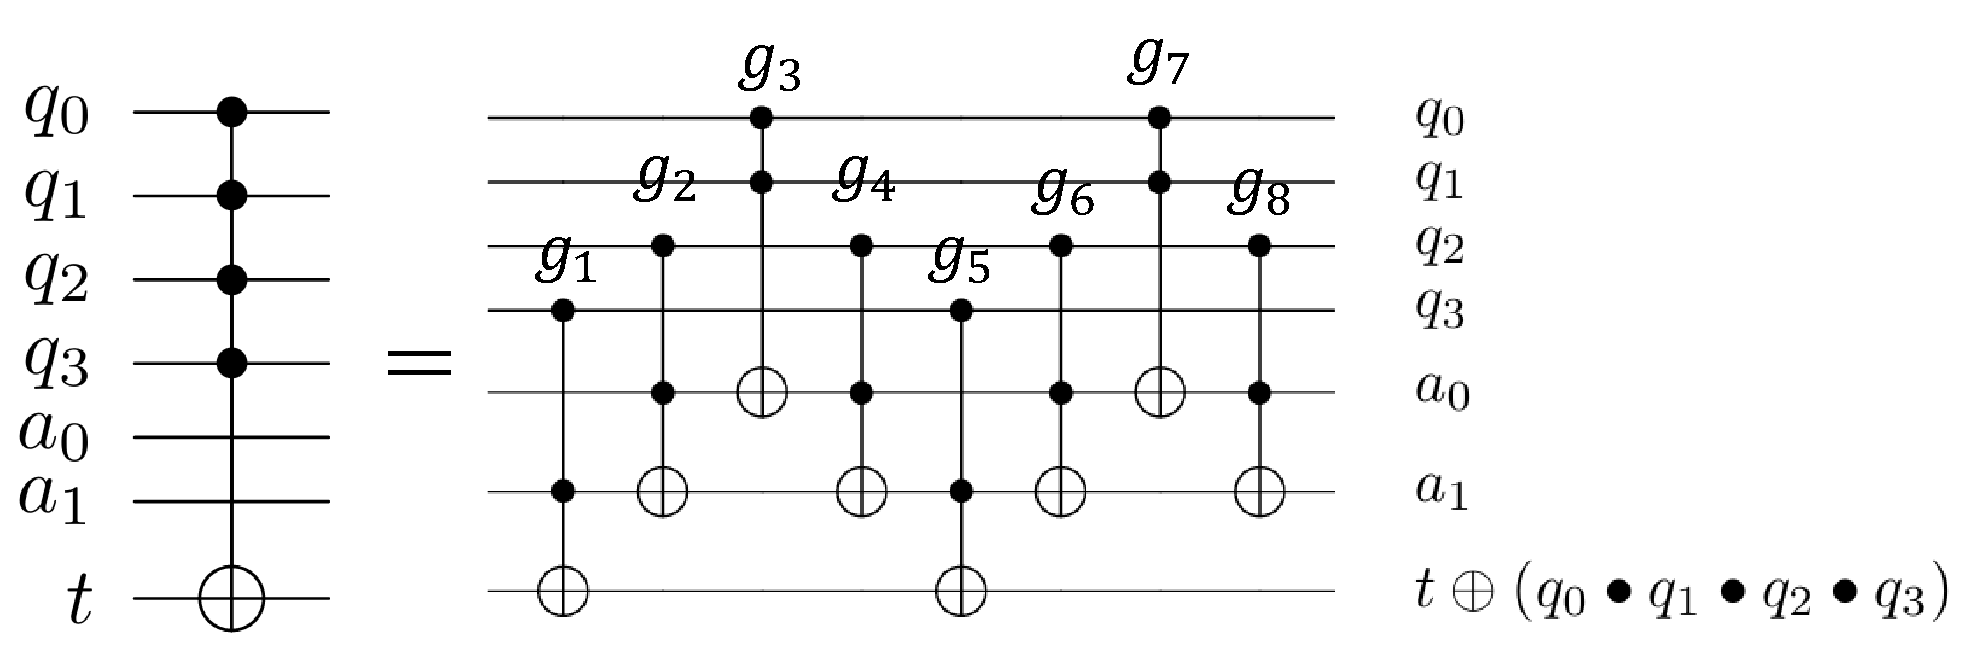
\includegraphics[width=13cm]{img/barenco.pdf}
  \caption{MCTゲートのToffoliゲートへの分解例}
  \label{barenco}
\end{figure}
図~\ref{barenco}では,MCTゲートを値が不定の補助ビット$a_{0},a_{1}$を用いて,Toffoliゲートへ分解している.
MCTゲートのコントロールビット数を$c$とすると,MCTゲートは$c-2$個の値が不定の補助ビットを用いて$4(c-2)$個のToffoliゲートに分解できる\cite{barenco1995elementary}.
図~\ref{barenco}の例では,コントロールビット数が4個のMCTゲートを2個の値が不定の補助ビットを用いて,8個のToffoliゲートに分解している.
\section{ビームサーチ}
ビームサーチ\cite{bisiani1992beam}は,
枝刈りをしながら木構造の探索をヒューリスティックに行う手法である.
木の深さが$M$,ノードからの遷移数を$N$とした場合,
すべての状態を調べると,$N^M$通りの状態をシミュレーションする必要がある.
$N$や$M$の値が大きい場合,
全ての状態をシミュレーションするのは現実的ではない.
そこで,探索範囲を事前に決めておいた数の候補に限定することで,
現実的な計算量に抑えて,探索を行う探索アルゴリズムがビームサーチである.
\par
ビームサーチでは,
事前に探索する深さと幅を指定してグラフの探索をする.
深さは,探索する木の高さ方向の大きさを意味する.
幅は,探索する木の横方向の大きさを意味する.
ビームサーチでは,指定した深さと幅を探索し,最良の候補を採用する.
Algorithm~\ref{alg:beam_search}にビームサーチ\bout{の疑似コードを示す.}
\begin{algorithm}[tbp]
  \caption{ビームサーチの疑似コード}
  \label{alg:beam_search}
  \begin{algorithmic}[1]
    \Require $state \Leftarrow$ 現在の状態
    \Require $legal\_actions$ 状態から次の遷移を列挙する関数  
    \Require $depth \Leftarrow$ 探索する深さ
    \Require $width \Leftarrow$ 探索する幅
    \State $best\_state$ 最良の候補
    \State $candidate\_list$ 探索候補のリスト,優先度付きキュー
    \State $candidate\_list.push(state)$
    \For{$1,..,depth$}
      \State $next\_candidate\_list$ 次の探索候補のリスト,優先度付きキュー
      \For{$1,..,width$}
      \If{$candidate\_list$が空なら}
        \State break
      \EndIf
      \State $now\_state \Leftarrow candidate\_list.pop()$ 探索候補の最良の値を取り出し,popする
      \State $next\_candidate\_list.push(legal\_actions(now\_state))$ 次の探索候補のリストに現在の状態からの遷移を追加
      \EndFor
      \State $candidate\_list \Leftarrow next\_candidate\_list$ 探索候補のリストを更新
      \State $best\_state \Leftarrow candidate\_list.top()$ 最良の候補を更新
      \If{$best\_state$が終了状態なら}
        \State break
      \EndIf
    \EndFor
    \State \Return $best\_state$の最初の遷移を返す
  \end{algorithmic}
\end{algorithm}

\begin{figure}[tbp]
  \centering
  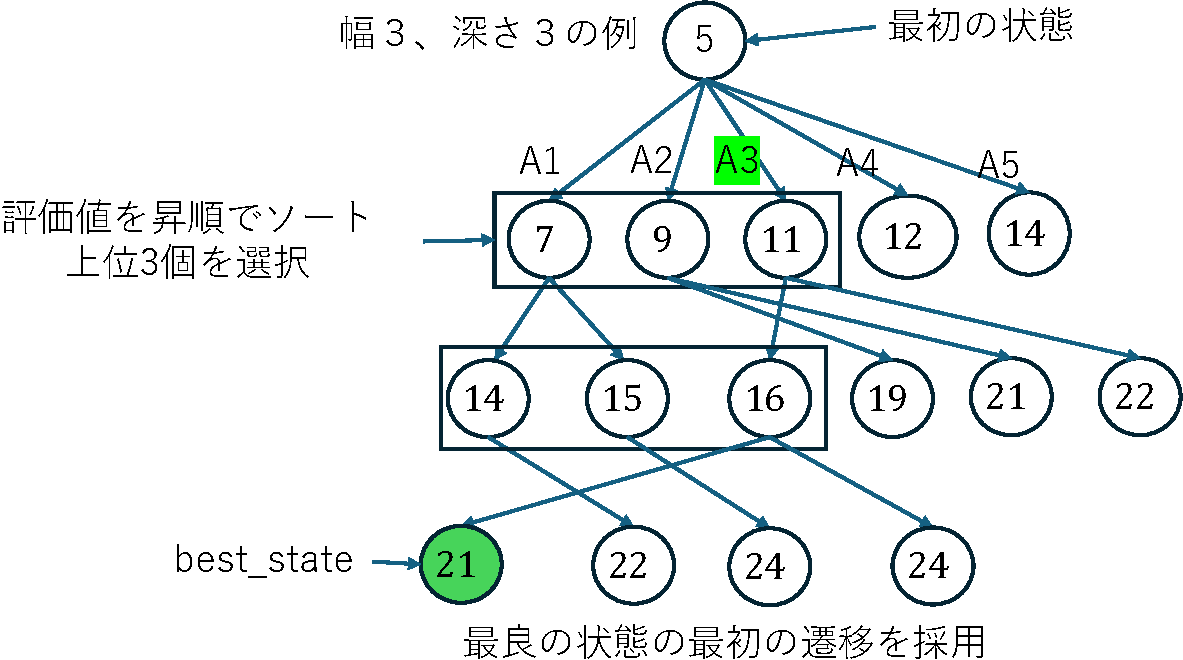
\includegraphics[width=11cm]{img/beam_search.pdf}
  \caption{深さ3,幅3の\gout{ビームサーチ}の動作例}
  \label{beam_search}
\end{figure}
図~\ref{beam_search}に深さ3,幅3の\gout{ビームサーチ}の動作例を示す.
図~\ref{beam_search}では,各ノードが状態を表している.
ノードに書かれている数字がその状態の評価値を表す.
\gout{図~\ref{beam_search}}の例では評価値が小さいものが優れた解であるとする.
初期状態からの状態の遷移をA1,A2,\dots ,A5とする.
図~\ref{beam_search}では初期状態から,5つの状態への遷移が列挙される.
探索する幅は3であるため,そのうち上位3個の状態を探索する.
上位3個の状態から\gout{遷移する状態を列挙し},再びその上位3個の状態を探索する.
この動作を繰り返し,深さ3に達したら,その時の最良の候補の最初の遷移A3を採用する.
